\section{Introduction and Examples}
\subsection{Tropical Arithmetic}
    \begin{definition} The tropical semiring $(\mathbb{R} \cup \{\infty\}, \oplus, \odot)$, is defined as the semiring whose underlying set is $\mathbb{R}$ with the binary operations: 
        \begin{align*}
            x \oplus y &= \text{min}(x,y)\\
            x \odot y  &= x + y
        \end{align*}
    We refer to $\oplus$ as the \textit{tropical sum}, and $\odot$ as the \textit{tropical product}. This can be a little confusing since the tropical product is defined as out usual notion of sum.
    \end{definition}

\subsection{Tropical plane curves}
Just like in algebraic geometry, our source of geometric objects in the tropical world comes from polynomials.
We will look at how polynomials behave on the tropical semiring to get an idea of the geometric objects we will soon be dealing with.
For any polynomial $f  = \sum_{i}c_{i}x^{i}\in \mathbb{R}[x]$, the standard polynomial ring, the tropical analougue, $\text{trop}(f)$ is:
\begin{align*}
    \text{trop}(f) &= \bigoplus_{i}c_{i}\odot x^{\odot i}\\
                   &= \text{min}_{i}(c_{i} + i \cdot x),
\end{align*}
a piecewise linear function from $\mathbb{R}$ to $\mathbb{R}$.

\begin{example}
    Consider the polynomial $f = x^{2} + x + 1$, then $\text{trop}(f) = \text{min}(2x,x,1)$. It's graph looks like the following.
    \begin{center}
        \begin{tikzpicture}
            \draw[blue] (0,0) -- (0.5,1);
            \draw[blue] (0.5,1) -- (1.5,2);
            \draw[blue] (1.5,2) -- (3,2);
            \draw[Stealth-Stealth] (0,1) -- (3,1) node [below]{x} -- (3.5,1);
            \draw[Stealth-Stealth] (0.5,0) -- (0.5, 2.8) node [left]{y} -- (0.5,3);
            \draw[-*](0,1) -- (1.5,1) node [below]{$(1,0)$};
            \draw[-*](0.5,0) -- (0.5,2) node [left]{$(0,1)$};
        \end{tikzpicture}
    \end{center}
    A piecewise linear polynomial.
\end{example}

\par Just like how we study the roots of polynomials in algrbaic geometry, in tropical geometry we care about the points in the domain where the tropical polynomial is \textit{not linear}.
This will be justified in remark \ref{rootValRmk} and the fundamental theorem in later sections.
\par The tropical polynomial in $2$ variables serve as a more instructive example to understand what the set of non-differentiable points look like. 

\begin{example}
    For a quadratic polynomial $f = ax^{2} + bxy + cy^{2} + dx + ey + g$, the tropicalisation looks like the tent aboce the plane in the figure below. 
    With the ``roots"" described earlier as the projection onto the plane below.
    \begin{figure}[ht]
        \centering
        \begin{tikzpicture}
            \node[inner sep = 0pt] at (0,0) {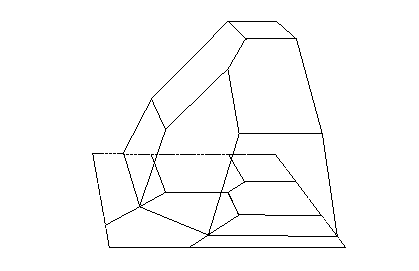
\includegraphics{Chapters/Images/tent.pdf}};
        \end{tikzpicture}
    \end{figure}
\end{example}

\begin{remark}
    \label{rmkOnTropPol}
    Note that the tropicalisation of polynomials in the rest of the thesis will be slightly different from the tropicalisations considered in this section.
    From now on we will be dealing with valuations and when we move the tropical world we will consider the valuations of the coeffiecients instead. 
    This will be elaborated upon in the next section.
\end{remark}

\subsection{Valuations and Varieties}
    \begin{definition}
        For a field $K$ we define the valuation $\emph{val}$ as a function $\emph{val}: K \to \mathbb{R}\cup \{\infty\}$ such that:
        \begin{enumerate}
            \item $\emph{val}(a) = \infty \Leftrightarrow a = 0$
            \item $\emph{val}(ab) = \emph{val}(a)+ \emph{val}(b)$
            \item $\emph{val(a+b)} \geq \emph{min}(\emph{val}(a),\emph{val}(b))$
        \end{enumerate}
        The image of $\emph{val}$ is an additive subgroup, $\Gamma_{\emph{val}} \subset \mathbb{R}$, called the value group.
        \par An important assumption we make is that $1 \in \Gamma_{\text{val}}$. 
    Further, we define $K^{\circ} := \{a \in K: \emph{val}(a)\geq 0\}$, and $K^{\circ \circ} := \{a \in K: \emph{val}(a)> 0\}$. 
    And the residue field $\tilde{K} := K^{\circ}/K^{\circ \circ}$.
    \end{definition}

    \begin{lemma}
        \label{vallemma}
        When $\text{val}(a) \neq \text{val}(b)$ for $a,b \in K$, then $\text{val}(a+b)= \text{min}(\text{val}(a),\text{val}(b))$.
    \end{lemma}
    It's not hard to see that the algebraic structure induced on the image of the valuation map is almost same as the algrbaic structure on the tropical semiring. 
    This observation motivates us to define tropicalisation of a polynomial with respect to a given valuation (as hinted in \ref{rmkOnTropPol}).
    For $f = \sum_{i}c_{i}x^{i} \in K[x]$ a polynomial in a valued field $(K, \text{val})$, the valued tropicalisation is defined as
    \begin{equation*}
        \text{trop}_{\text{val}}(f) = \text{min}_{i}(\text{val}(c_{i}) + i \cdot x).
    \end{equation*}
    \begin{remark}
        \label{rootValRmk}
    We now make a key observation. For any tropical polynomial (tropicalisation of a standard polynomial) in one variable, we refer to the points where it's not differentiable as its \textbf{roots}. 
    Suppose $f(x) = \prod_{i=1}^{n}(x-\lambda_i) \in K[x]$, where $K$ is some valued field, then $\text{trop}(f) = \sum_{i=1}^{n}\text{min}(\text{val}(x),\text{val}(\lambda_i))$. 
    It's clear that the \textbf{``roots"} of $\text{trop}(f)$ are $\text{val}(\lambda_i)$.
    This relation between the two types of \textit{roots} will be further generalised, and will lead to the \textit{fundamental theorem of tropical geometry}.
    \end{remark}

    \begin{lemma}
        Suppose $K$ is an algebraically closed valued field, then the value group $\Gamma_{\emph{val}}$ is divisible and dense in $\mathbb{R}$.
    \end{lemma}

    \begin{lemma}
        When $K$ is an algebraically closed valued field, the surjection $K^{*} \twoheadrightarrow \Gamma_{\emph{val}}$ splits.
    \end{lemma}

    The splitting is a map $\phi: \Gamma_{\text{val}} \to K^{*}$, but we always denote $\phi(w)$ with $t^w$. This notation is inspired from the splitting in the case where $K$ is the field of Puiseux series.
    \par Other than the standard affine and projective spaces, in tropical geometry we often deal with \textit{n-dimensional algebraic tori}: $T^{n}_{K} := T^n = (K^{*})^n$. 
    The coordinate ring of $T^{n}$ is $K[x_{1}^{\pm 1},\dots,x_{n}^{\pm 1}]$, the ring of laurent polynomials. 
    Zero set of ideals in the laurent polynomial ring define varieties in $T^n$, these varieties are called \textbf{very affine varieties}.
    Just like for affine spaces we can define a Zariski topology on $T^{n}$.
    \par We now have the inclusions $i: T^{n} \hookrightarrow \mathbb{A}^n$ and $j: \mathbb{A}^{n} \hookrightarrow \mathbb{P}^{n}$. 
    The affine closure of a very affine variety $X$ is $\overline{i(X)}$, and the projective closure of a affine variety $X$ is $\overline{j(X)}$. 
    For an ideal $I \subset K[x_{1}^{\pm 1},\dots,x_{n}^{\pm 1}]$, define $I_{\text{aff}}:= I \cap K[x_{1},\dots,x_{n}]$.

    \begin{proposition}
        For $I \subset K[x_{1}^{\pm 1},\dots,x_{n}^{\pm 1}]$ let $X = V(I) \subset T^n$, then $V(I_{\text{aff}}) = \overline{i(X)}$.
    \end{proposition}

    \begin{proposition}
        \label{densenessprop}
        $(K,v)$ be a valued field with splitting $\Gamma_{\emph{val}} \twoheadrightarrow \mathbb{R},~w \to t^{w}$.
        Let $\alpha_{1}, \dots,\alpha_{n} \in \tilde{K}^{*}$ and $w_1, \dots, w_n \in \Gamma_{\emph{val}}$. 
        Conisder the set of $\textbf{y} = (y_1, \dots, y_n) \in T^{n}$ such that $\emph{val}(y_{i}) = w_{i}$ and $\overline{t^{-w_i}y_i} = \alpha_{i}$ for all $1\leq i \leq n$.
        This set is dense in $T^n$ with respect to the Zariski topology.
    \end{proposition}

    \subsection{Polyhedral Geometry}
We now very quickly go through some elementray definitions and constructions in Polyhedral Geometry. 
This section very closely follows the exposition in section 2.3 of \cite{maclagan2015introduction}.
   \par A set $X\subset \mathbb{R}^{n}$ is said to be \textbf{convex} if for any two points in $X$ the line connecting those two points also lies in $X$. 
   The \textbf{convex hull}, conv$(U)$, of a set $U\subset \mathbb{R}^{n}$ is the smallest convex set containg $U$.
   When $U$ is a finite set $\text{conv}(U)$ is a \textbf{polytope}. 
   A \textbf{polyhedral cone} $C \subset \mathbb{R}^{n}$ is the \textit{positive hull} of a finite subset of $\mathbb{R}^{n}$. 
   For a set $U = \{u_1,\dots,u_n\}$:
   \begin{align*}
       C = \text{pos}(U) = \left\{\sum_{i=1}^{n}\lambda_i u_i~:~\lambda_i\geq 0\right\}
   \end{align*}
   When the $u_i$'s are linearly independent, the cone is said to be \textbf{simpilicial}. 
    It's easy to see that every polyhedral cone is a finite intersection of \textit{half n-spaces}, this perspective allows to define cones as the set $\{x \in \mathbb{R}^{n}: Ax\leq 0\}$, where $A$ is a $d \times n$ matrix. 
    For a dual vector $w \in (\mathbb{R}^{n})^{\vee}$ we define the associated face in the cone $C$ as:
    \begin{align*}
        \text{face}_{w}(C) = \left\{x \in C: w\cdot x \leq w\cdot y ~\text{for all}~y \in C\right\}
    \end{align*}
    For $d'$ the dimension of the face, there also exists a $d'\times n$ matrix $A'$ such that $\{x \in C: A'x\ =  0\}$. 
    A \textbf{polyhedral fan} is a collection of polyhedral cones such that every face of the cone is part of the collection, and the intersection of any two cones is a face of both the cones.
    A \textbf{polyhedron} $P \subset \mathbb{R}^{n}$ is the intersection of finitely many affine half spaces, allowing us to define it as the set $\{x \in \mathbb{R}^{n}: Ax\leq b\}$ where $b \in \mathbb{R}^{d}$ and $A$ is a $d \times n$ matrix. We can define faces of polyhedron's in the same manner as we defined faces of a cone.
    \par A \textbf{polyhedral complex}, $\Sigma$, is a collection of polyhedron such that: if $P \in \Sigma$ then all faces of $P$ also lie in $\Sigma$, and if $P,Q \in \Sigma$ then $P \cap Q = \emptyset$ or $P \cap Q$ is a face of both $P,Q$. The support of a polyhedral complex, $|\Sigma |$ is the underlying set of points in $\Sigma$. 
    The \textbf{lineality space} of a polyhedral complex, if it exists, is the largest linear subspace which lies in it.
    For any set of points in $\mathbb{R}^{n}$, their \textbf{affine span} is defined as the smallest affine subspace containing those points.

    The \textbf{regular subdivision} is an important construction since it helps us create a link between the newton polytope and tropical variety. 
    \begin{definition}
    For an ordered list of vectors $v_1,\dots, v_r \in \mathbb{R}^{n}$, fix a weight vector $w = (w_1,\dots,w_n) \in \mathbb{R}^{n}$. 
    The \textit{regular subdivision} is the polyhedral fan with support $\text{pos}(v_1,\dots,v_n)$ whose cones are $\text{pos}(\sigma)$ for all $\sigma \subset \{v_1,\dots,v_n\}$ such that there exists $c \in \mathbb{R}^{n+1}$ for which:
    \begin{itemize}
        \item $c \cdot v_i = w_i$ for all $v_{i}\in \sigma$ 
        \item $c \cdot v_i < w_i$ for all $v_i \not\in \sigma$
    \end{itemize}
    Although defined as a fan, regular subdivisions are usually defined for polyhedral complexes.
    \end{definition}
    Suppose you have a polyhedron $P$ given by $\text{conv}(u_i: 1\leq i\leq r)$, we look at the vectors $v_i = (u_i,1)$. 
    The regular subdivision of $v_1,\dots,v_r$ with respect to a weight vector $w = (w_1, \cdots, w_r)$ can be interpreted as projection of the bottom faces of the polytope $P_w = \text{conv}\{(u_i,w_i): 1\leq i\leq r\}$. 
    That is, in the polytope $P_w$ consider the faces $F$ whose normal vector has positive final coordinates and project them onto the first $r$ coordinates, this gives the regular subdivision of $P$ with respect to $w$.

\section{Tropical Hypersurfaces}

    \begin{definition}
        Consider polynomial $f = \sum c_u x^u \in K[x_0,\dots,x_n]$, and let
        \[
            W = \text{trop}(f)(w) = \text{min}_{u \in \mathbb{Z}^{n+1}}\{\text{val}(c_u) + u\cdot w\}.
        \]
        Then we define the initial form of $f$ with respect to $w$ as
        \begin{align*}
            \text{in}_{w}(f)(x) = \sum_{\text{val}(c_u) + u\cdot w = W} \overline{c_u t^{-\text{val}(c_u)}} x^u.
        \end{align*}
        We can also define the initial form for a laurent polynomial $f$ in the same way.
    \end{definition}

    It's easter to discuss properties of these initial forms once we understand their relation to tropical hypersurfaces.
    So before we further study these intial forms, we will first look at tropical hypersurfaces.
    \begin{definition}
        For a laurent polynomial $f \in  K[x_{1}^{\pm1}, \dots, x_{n}^{\pm1}] $, the tropical hypersurface $\emph{trop}(V(f))$ is the set:
        \begin{align*}
        \{w \in \mathbb{R}^{n}: \text{minimum in }\emph{trop}(f)(w)\text{ is acheived atleast twice}\}.
        \end{align*}
    \end{definition}
    Similarly, for a tropical polynomial $F$, $V(F)$ denotes the set:
    \begin{align*}
        \{w \in \mathbb{R}^{n}: \text{minimum in }F(w)\text{ is acheived atleast twice}\}.
    \end{align*}
    It's clear that for a laurent polynomial $f$: $V(\text{trop}(f)) = \text{trop}(V(f))$

    That next theorem gives various characterisations for a tropical hypersurface.
    The generalisation of this theorem to varieties of higher codimensions is called the \textit{fundamental theorem of Tropical Geometry}.
    \begin{theorem}[Kapranov's Theorem]
    Let $K$ be an algebraically closed field with a non-trivial valuation. Fix a laurent polynomial $f \in K[x_{1}^{\pm1}, \dots, x_{n}^{\pm1}]$. The following sets are the same:
    \begin{enumerate}
        \item $A$ = $V(\text{trop}(f))$.
        \item $B$ = $\{w \in \mathbb{R}^{n}: \text{in}_{w}(f)~ \text{is not a monomial}\}$.
        \item $C$ = closure of $\left\{(\text{val}(y_1), \dots, \text{val}(y_n)): (y_1,\dots, y_n) \in V(f)\right\}$ in $\mathbb{R}^{n}$.
    \end{enumerate}
    Further, if $f$ is irreducible and $w \in \Gamma_{\text{val}} \cap \text{trop}(V(f))$, then the set $\{y \in V(f): \text{val}(y) = w\}$ is Zariski dense in $V(f)$.
    \end{theorem}

    \begin{proof}[Sketch of proof]
        Showing $A$ = $B$ is straightforward. 
        If $x \in A$ then there exist atleast two $u_1,~u_2$ such that $\text{trop}(f)(x) = \text{val}(c_{u_{1}}) + u_{1}\cdot x = \text{val}(c_{u_{2}}) + u_{2}\cdot x$. 
        This implies $\text{in}_{x}(f)$ has atleast the terms corresponding to $u_1$ and $u_2$, implying it's not a monomial, and $A \subset B$.
        Now consider a $w \in B$, the initial form $\text{in}_{w}f = \sum_i \text{val}(c_{u_{i}}) + u_i \cdot w$ has atleast two terms, say for $i=1,2$. 
        Therefore $\text{trop}(f)(w) = \text{val}(c_{u_{1}}) + u_{1}\cdot w = \text{val}(c_{u_{2}}) + u_{2}\cdot w$, implying $w \in A$.
        Hence A = B.
        \par To show $C \subset A$, since $A$ is already closed, we just need to show that the set $\{(\text{val}(y_1), \dots, \text{val}(y_n)): (y_1,\dots, y_n) \in \mathbb{R}^{n}\}$ lies in $A$. Say $\textbf{y} = (y_1,\dots,y_n) \in V(f)$, this implies 
        \begin{align*}
            f(\textbf{y}) &= \sum_u c_u y^{u} = 0 \\
            \Rightarrow&\text{val}(\sum_u c_u y^{u}) = \infty \\
            \Rightarrow& \text{min}_u(\text{val}(c_u) + u \cdot \text{val(\textbf{y})}) = \infty
        \end{align*}
        For this equality to hold, for any pair $u_{1},~u_{2}$ with $c_{u_{i} \neq 0}$ we need to have $\text{val}(c_1) = \text{val}(c_2)$, else by [\ref{vallemma}] $\text{val}(f(\textbf{y})) < \infty$, which is a contradiction. 
        \par To finish of the proof, we show $B \subset C$ and the density statement in the next propostion.
    \end{proof}
    This proposition uses notation from the statement of Kapranov's Theorem.
    \begin{proposition}
        Fix a laurent polynomial $f \in  K[x_{1}^{\pm1}, \dots, x_{n}^{\pm1}]$, and let $w \in \Gamma_{\text{val}^{n}}$. 
        Suppose $w \in B$ and $\alpha \in (\tilde{K}^{*})^{n}$ satisfies $\text{in}_{w}(f)(\alpha) = 0$. 
        There exists $\textbf{y} \in (K^{*})^{n}$ such that $f(\textbf{y}) = 0$,  $\text{val}(\textbf{y}) = \textbf{w}$, and $t^{-1_{i}}y_{i}=\alpha_{i}$ for $1 \leq i \leq n$.
        Further, if $f$ is irreducible, then the set of such $\textbf{y}$ is Zariski dense in the hypersurface $V(f)$.
    \end{proposition}
    \begin{proof}
        We go about proving this proposition via induction on $n$.
        \par \textit{Base Case.} Consider $n = 1$.
        \par We can multiply by a unit and assume that $f = \sum_{i=0}^{s}c_{i}x^{i}$ such that $c_{0}, c_{s}\neq0$. 
        Since we are working in an algebraically closed field $K$, $f = \prod^{s}_{j=1} (a_{j}x-b_{j})$. 
        Then, $\text{in}_{w}(f) = \prod^{s}_{j=1} \text{in}_{w}(a_{j}x-b_{j})$. 
        Since $\alpha \in \tilde{K}$ and $\text{in}_{w}f(\alpha)=0$, there exists $j$ such that $\text{in}_{w}(a_{j}x-b_{j})(\alpha) = 0$.
        Futher, since $w \in B$, the initial form $\text{in}_{w}(f)$ is not a monomial.
        This implies that $\text{in}_{w}(a_{j}x-b_{j})$ is not a monomial, hence:
        \begin{align*}
            \text{val}(a_{j}) + w &= \text{val}(b_{j})\\
            \alpha &= \overline{t^{-w}b_{j}/a_{j}}.
        \end{align*}
        Setting $y = b_{j}/a_{j}$ we get $f(y) = 0$, and $\overline{t^{-\text{val}(y)}y} = \alpha$, proving the base case.
        \par \textit{Inducting on n}. Consider $n>1$.       
        We first show that there exists an automorphism on $\phi \in K[x_{1}^{\pm1}, \dots, x_{n}^{\pm1}]$ such that $\phi(f)$, when seen as a polynomial in $x_{n}$, has coefficients which are monomials in $ K[x_{1}^{\pm1}, \dots, x_{n-1}^{\pm1}]$. 
        It's easy to construct such a automorphism:
        \begin{itemize}
            \item Choose $l \in \mathbb{Z}_{>0}$.
            \item Define $\phi^{*}_{l}: K[x_{1}^{\pm1}, \dots, x_{n}^{\pm1}] \to  K[x_{1}^{\pm1}, \dots, x_{n}^{\pm1}]$ as:
                \begin{align*}
                    x_{i} &\mapsto x_{i}x_{n}^{l^{i}}~~\text{for }1\leq i\leq n-1\\
                    x_{n} &\mapsto x_{n}.
                \end{align*}
            \item Any monomial in the polynomial $f$ can be expressed as $x^{\textbf{u}}x_{n}^{r}$, where $\textbf{u} \in \mathbb{Z}^{n-1}$, and:
                \[
                    \phi^{*}_{l}(x^{\textbf{u}}x_{n}^{r}) = x^{\textbf{u}}x_{n}^{r+\sum_{i=1}^{n-1}l_{i}}.
                \]
            \item It's clear now that we can choose $l$ large enough such that each monomial of $f$ under $\phi^{*}_{l}$ has a unique exponent in $x_{n}$.
        \end{itemize}
        \par Hence, we have found an automorphism $\phi^{*}_{l}$ which satisfies the required propeties. If $\textbf{y}\in T^{n}$ satisfies:
        \begin{align*}
            \phi^{*}_{l}(f)(\textbf{y}) &= 0\\
            \text{val}({y}_{i}) &= w_{i} - l^{i}w_{n} \\
            \overline{t^{-w_{i}- l^{i}w_{n}}y_{i}} &= \alpha_{i}\alpha_{n}^{-l^{i}},
        \end{align*}
        then for  $\textbf{y}'\in T^{n}$, defined by $y'_{i}=y_{i}y_{n}^{l^{i}}$ for $1\leq i<n$, and $y'_{n}  = y_{n}$:
        \begin{align*}
            f(\textbf{y}') &= 0\\
            \text{val}({y'}_{i}) &= w_{i} \\
            \overline{t^{-w_{i}}y'_{i}} &= \alpha_{i}.
        \end{align*}
        Therefore we can replace $f$ with $\phi^{*}_{l}(f)$.
        By construction of $\phi^{*}_{l}$, we know that when $f$ is regarded as a polynomial in $x_{n}$, all coefficients are monomials in $ K[x_{1}^{\pm1}, \dots, x_{n-1}^{\pm1}]$.
        \par Consider the set $\mathcal{V} := \{(y_{1},\dots, y_{n-1})\in T^{n-1}: \text{val}(y_{i}) = w_{i},\,\overline{ t^{-w_{i}}y_{i}} = \alpha_{i} \}$.
        From proposition \ref{densenessprop}, we know that the set $\mathcal{V}$ is Zariski dense in $T^{n-1}$.
        Additionaly, for each such point $\textbf{y}\in \mathcal{Y}$ the polyomial defined by $g(x_{n}) = f(y_{1},\dots, y_{n-1}, x_{n})$ is non-zero.
        For $\textbf{u} \in \mathbb{Z}^{n}$ we denote with $\textbf{u}'\in \mathbb{Z}^{n-1}$ the projection of $\textbf{u}$ onto the first $n-1$ coordinates. 
        \par With $\textbf{u} = (\textbf{u}',i)$, the polynomial $g$ has the form,
        \begin{align*}
            g(x_{n}) = \sum_{i} c_{\textbf{u}}\textbf{y}^{\textbf{u}'}x_{n}^{i}
        \end{align*}
        And for each monomial corresponding to $\textbf{u}$ we have:
        \begin{align*}
            &~ \text{val}(c_{\textbf{u}}) + \text{val}(\textbf{y}^{\textbf{u}'}) + w_{n}\cdot i\\
            =& ~\text{val}(c_{\textbf{u}}) + \textbf{w} \cdot \textbf{u}.
        \end{align*}
        Therefore, $\text{trop}(g)(w_{n}) = \text{trop}(f)(\textbf{w})$, implying:
        \begin{align*}
            \text{in}_{w_{n}}(g)(x_{n}) =& \sum_{\substack{\textbf{u}:\, \text{val}(c_{\textbf{u}}) + \text{val}(\textbf{y}^{\textbf{u}'}) \\+ w_{n}\cdot u_{n} = \text{trop}(g)(w_{n})}} \overline{t^{-\text{val}(c_{\textbf{u}})}c_{\textbf{u}}t^{-\textbf{u}'\cdot \textbf{w}'}y^{\textbf{u}'}}x^{u_n}_{n} \\
            =& \sum_{\substack{\textbf{u}:\, \text{val}(c_{\textbf{u}}) + \textbf{w} \cdot \textbf{u} \\= \text{trop}(g)(w_{n})}}\overline{t_{-\text{val}(c_{\textbf{u}})}c_{\textbf{u}}}\alpha^{\textbf{u}'}x^{u_{n}}_{n}\\
            =& ~ \text{in}_{\textbf{w}}(f)(\alpha_{1}, \dots, \alpha_{n-1}, x_{n}).
        \end{align*}
        So from $\text{in}_{\textbf{w}}(f)(\alpha) = 0$ we get $\text{in}_{w_{n}}(g)(\alpha_{n}) = 0$.
        From the $n=1$ case there exists a $y_{n} \in K^{*}$ such that $\text{val}(y_n) = w_n$, $\overline{t^{-\text{val}(w_{n})}y_{n}} = \alpha_{n}$, and $g(y_{n}) = 0$, implying $f(y_1,\dots,y_n) = 0$.
        Therefore, we have found the required point $y \in V(f)$.
        \par We are now left with the last claim of the proposition - if $f$ is an irreducible polynomial the set $\mathcal{Y} = \{\textbf{y}\in V(f): \text{val}(\textbf{y}) = \textbf{w},\, \overline{t^{-w_{i}}y_{i}} = \alpha_{i},\, 1\leq i\leq n\}$ is dense in $V(f)$.
        For each point $(y_{1},\dots, y_{n-1}) \in \mathcal{V}$ we constructed a point $\textbf{y} = (y_{1},\dots, y_{n-1}, y_{n}) \in \mathcal{Y}$.
        Now consider any $g \in I(\mathcal{Y})$ (that is $g(y)= 0$ for all $y \in \mathcal{Y}$), if we show that $g\in \langle f \rangle$, then denseness follows.
        We know that $\mathcal{V}$ is dense in $T^{n-1}$.
        As a consequence, the projection of $\mathcal{Y}$ onto the first $n-1$ coordinates can't be the solution set of any polynomial in $ K[x_{1}^{\pm1}, \dots, x_{n-1}^{\pm1}]$.
        Hence, the ideal $\langle f,g \rangle$ contains no non-trivial polynomial in $ K[x_{1}^{\pm1}, \dots, x_{n-1}^{\pm1}]$.
        Since $f$ is irreducible, it follows that $g = h \cdot f$ for some laurent polynomial $f$, implying $g \in\langle f \rangle$.
        Therefore, $\mathcal{Y}$ is dense in $V(f)$.
    \end{proof}

    \begin{theorem}
        \label{trpisNewtTh}
        For $f \in K[x_1^{\pm 1}, \dots, x_n^{\pm 1}]$, and $\text{trop}(V(f)) = |\Delta|$. Where $\Delta$ is a pure $\Gamma_{val}^n-$rational polyhedral complex of dimension $n-1$, more specifically:
        \begin{equation*}
            \Delta = \left(\text{dual}\left(\text{r-subdiv}_{\text{val}(c_u)}\left(\text{Newt}(f)\right)\right)\right)^{[n-1]}
        \end{equation*}
    \end{theorem}
    \begin{proof} 
       Let $f = \sum_{u \in \mathbb{Z}^n}c_ux^u$
       \begin{itemize}
           \item $P = \text{conv}\{u: c_u \neq 0\} \subset \mathbb{R}^n$ .
           \item $P_{\text{val}} = \text{conv}\{(u,c_u): c_u \neq 0\}\subset \mathbb{R}^{n+1}$.
       \end{itemize}
       Defining the following will be helpful:
       \begin{itemize}
           \item $\text{face}_v(P) = \{x \in P : x\cdot v \leq y \cdot v~ \text{for all } y \in P\}$. Here the vector $v$ is an inward pointing normal vector of the face.
           \item $\pi: \mathbb{R}^{n+1} \to \mathbb{R}^n$ projection onto first $n$-coords.
       \end{itemize}
       The regular subdivision of $P$ with weight vectors given by $c_u$ is the projection of the lower faces of $P_{\text{val}}$.
       A face is called a \textit{lower face} if it can be defined with a vector $v$ for which $v_{n+1} > 0$.
       
       Now that we have the regular subdivision, we define the dual:
       \begin{itemize}
           \item The \textit{Normal Cone} of a face is the set of all defining vectors of the face.
               Formally, for a face $F \subset P_{\text{val}}$, the \textit{Normal Cone} $\mathcal{N}(F) = \{v \in \mathbb{R}^{n+1}: \text{face}_v(P_{\text{val}}) = F\}$.
           \item And $\mathcal{F} = \{v \in \mathcal{N}(F): v_{n+1} = 1\}$.
           \item $\tilde{\pi}(F) = \pi(\mathcal{F})$
       \end{itemize}
       And the complex $D = \{\tilde{\pi}(F) : F \text{ is a lower face of }P_{\text{val}}\}$ defines the dual of the regular subdivision. 
       Let's see what the initial form defined by $v \in \tilde{\pi}(F)$ looks like (let $\bar{v} = (v,1) \in \mathcal{F}$ be the pre-image of $v$).
       \begin{align*}
           \text{in}_v(f) = \sum_{\text{val}(c_u) + v \cdot u = w} \overline{c_u t^{-\text{val}(c_u)}} x^u
       \end{align*}
       Where $w = \text{min}_{u}\{\text{val}(c_u) + u\cdot v\}$. 
       Notice $\text{val}(c_u) + v \cdot u = \bar v \cdot (u,c_u)$, 
       so if $x^{u'}$ has non-zero coefficient in $\text{in}_v(f)$: 
       \begin{equation*}
           (u',c_{u'})\cdot \bar{v} \leq (u,c_u) \cdot \bar{v}~~~\forall u
       \end{equation*}
       Which is precisely the condition required for $(u,c_u)$ to be a vertex of the face F defined by $\bar v$, and consequently for $u$ to be vertex of $\pi(F)$. 
       Therefore $\text{in}_{v}(f)$ is \textit{not} a monomial \textbf{iff} $\text{face}_v(P_{val})$ has more than vertex.
       \par So $w\in \text{trop}(f)(v)$ \textbf{iff} $\text{face}_{(w,1)}(P_{val})$ is a \textit{not} a vertex. 
       Implying, $w \in D^{[n-1]}$.
   \end{proof}

\section{Gr\"{o}bner and Tropical Bases}  
Kapranov's theorem hints at the fact that the set of weights used to define the initial forms for a laurent polynomial have some additional structure. 
Over the course of this section we will see that for an ideal $I$ the set of weights which induce a non-trivial ideal of initial forms has the structure of a $\Gamma_{\text{val}}-$raitonal polyhedral complex.

\par Before we develop the theory of initial forms of laurent polynomials, we will look at initial forms for homogenous polynomials (and ideals). 
The reasoning behind this is explained in remark \ref{whyHomoRmk}.

\begin{definition}
    For a homogenous ideal $I$ the initial ideal $\text{in}_{w}(I)$ is defined as the ideal in $\tilde{K}[x_0,\dots,x_n]$ generated by intial forms of polynomials in $I$. 
    A set $\mathcal{G} \subset I$ is called a groebner basis of $I$ with respect to $w$ if $\langle\text{in}_{w}\left(\mathcal{G}\right)\rangle = \text{in}_{w}(I)$.
\end{definition}

    \begin{lemma}
        $I \subset K[x_0,\dots, x_n]$ be a homogenous ideal; fix $w\in \mathbb{R}^{n+1}$. 
        Then $\text{in}_{w}(I)$ is a homogenous ideal, and there exists a homogenous greobner basis for $I$. 
        Further, if $w \in \Gamma_{\text{val}}$ then $g \in \text{in}_{w}(I)$ has the form $g = \text{in}_{w}(f)$ for $f \in I$.
    \end{lemma}

    \begin{remark}
        \label{whyHomoRmk}
        The reason we are dealing with homogenous ideals is because unlike standard gr\"{o}bner basis theory the ordering of monomials is also dependent on the (valuations of the) coefficients. 
        This implies that gr\"{o}bner bases needn't always generate the original ideal like usual. But when the ideals are homogenous, the gr\"{o}bner basis generates the original ideal.
    \end{remark}

    \begin{lemma}
        For a fixed polynomial $f \in K[x_0,\dots,x_n]$ and $w,v \in \mathbb{R}^{n+1}$ there exists $\varepsilon >0$ such that for all $0<\varepsilon ' < \varepsilon$: 
        \begin{equation*}
            \text{in}_{v}(\text{in}_{w}(f)) = \text{in}_{w + \varepsilon 'v}(f).
        \end{equation*}
    \end{lemma}
    \begin{remark}
    The previous lemma should be interpreted in a geometric context.
    From Kapranov's theorem we know that the set of weights of initial forms has the structure of a polyhedral complex. 
    Therefore, the above lemma implies that when take the initial form of the initial form ($\text{in}_{v}(\text{in}_{w}(f))$), it's equivalent to initialising just once at a point close to $w$ in the polyhedral complex of weights.
    This is infact also true at the level of Ideals - formalised in the next proposition.
    \end{remark}

    \begin{proposition}
        \label{ininIdeal}
        For a homogeonous ideal $I \in K[x_0,\dots,x_n]$ and $w,v \in \mathbb{R}^{n+1}$ there exists $\varepsilon >0$ such that for all $0<\varepsilon ' < \varepsilon$:
        \begin{equation*}
            \text{in}_{v}(\text{in}_{w}(I)) = \text{in}_{w + \varepsilon 'v}(I).
        \end{equation*}
    \end{proposition}

    \begin{lemma}
        If $I \subset K[x_0,\dots,x_n]$ is a homogenous prime ideal of dimension $d$ and $w \in \Gamma_{\text{val}}^{n+1}$, then every minimal associated prime of $\text{in}_{w}(I)$ has dimension $d$.
    \end{lemma}

\subsection{Gr\"{o}bner Complexes}

We now build towards generalising Kapranov's theorem to abritary very affine varieties.
We continue to work with homogenous ideals over a field which admits a splitting, and in the next section we will move to the ring of laurent polynomials.

\begin{definition}
    Consider a homogenous ideal $I \subset K[x_{0},\dots, x_{n}]$.
For each $w \in \Gamma_{\text{val}}^{n+1}$ we define the polyhedra:
\begin{equation*}
    C_{I}[w] := \{w' \in \mathbb{R}^{n+1}: \text{in}_{w}(I) = \text{in}_{w'}(I)\}.
\end{equation*}
    The closure of this set with respect to the euclidean topology is given by $\overline{C_{I}[w]}$.
\end{definition}

\begin{proposition}
    \label{finInIdProp}
    $I\subset K[x_{0},\dots,x_{n}]$ be a homogenous ideal.
    There exist only finitely many distinct monomial ideal $\text{in}_{w}(I)$ as $w$ varies over $\mathbb{R}^{n+1}$.
\end{proposition}

\begin{remark}
    \label{facePolyRmk}
If for $w \in \mathbb{R}^{n+1}$ the ideal $\text{in}_{w}(I)$ is not a monomial ideal, there exists a $w'\in \mathbb{R}^{n+1}$, such that:
\begin{itemize}
    \item $\text{in}_{w'}(I)$ is a monomial ideal.
    \item $\overline{C_{I}[w']}$ is a proper face of the polyhedra $\overline{C_{I}[w]}$.
\end{itemize}
Additionaly, the set $\overline{C_{I}[w]}$ is a $\Gamma_{\text{val}}$-rational polyhedron, with a lineality space given by $\mathbb{R}\textbf{1}:= \text{span}\{(1,1,\dots,1)\}$. 
We refer the reader to theorem 2.5.2 of \cite{maclagan2015introduction} for the proof of this claim.
\par Since we don't care about the lineality space, we identify with $\overline{C_{I}[w]}$ the space $\overline{C_{I}[w]} / \mathbb{R}\textbf{1}$. 
As we vary $w$ across $\mathbb{R}^{n+1}$, we can glue $\overline{C_{I}[w]}$ to from a polyhedral comples - we prove this in theorem \ref{grobCompThe}.
\end{remark}

\begin{definition}
    Let $F: \mathbb{R}^{n+1}\to \mathbb{R}$ be a tropical polynomial function, we denote with $\Sigma_{F}$ the coarsest polyhedral complex, such that $F$ is linear on each cell of $\Sigma_{F}$.
    The maximal cells of $\Sigma_{F}$ is of the form $\sigma = \{w \in \mathbb{R}^{n+1}: F(w) = a + w \cdot u\}$, where $a\odot x^{\odot u}$ is an element in the polynomial $F$.
\end{definition}

\begin{remark}
    Given an ideal $I$ we can construct a polynomial $g$ such that if $w \in \text{relint}(\sigma)$ where $\sigma$ is a maximal cell of $\Sigma_{\text{trop}(g)}$, then $\sigma = \overline{C_I[w]}$ for $w \in \mathbb{R}^{n+1}$. 
    We now describe the construction of the polynomial $g$. 
    \begin{itemize}
        \item For a $r \times s$ matrix $A$, and a cardinality $r$ subset $J$ of the set of columns of $A$, we denote with $A^{J}$ the $r \times r$ submatrix corresponding to the columns indexed by $J$.
        \item Let $I \subset K[x_{0}, \dots, x_{n}]$ be a homogenours ideal, and for $d \in \mathbb{Z}_{>0}$, let $\mathcal{S}_{d}:=\{f_{1},\dots, f_{r}\}$ be a basis for $K$-the submodule $I_{d}\subset I$ of degree $d$ elements of $I$.
        \item We know that every homogenous polynomial of degree $d$ on $n+1$ variables has $\binom{n+d}{n}$ coefficients. 
            Let $H_{d}$ be an indexing set for the $\binom{n+d}{n}$ coefficients.
            Let $A_{d}$ be a $r \times \binom{n+d}{n}$ matrix, with rows indexed by $\mathcal{S}_{d}$ and columns indexed by $H_{d}$; thus, $A_{ij}$ is the $j^{\text{th}}$ coefficient of the polynomial $f_{i}$.
        \item Consider the vector:
            \begin{align*}
                P(I_{d}) := (\text{det}(A_{d}^{J}))_{ J \in \{{J \subset H_{d}: |J| = r}\}}.
            \end{align*}
            We call $P(I_{d})$ the Pl\"{u}cker coodrinates of the point $I_{d}$ in the grassmanian $G(r, H_{d})$ (space of dimension $r$ subspaces in $|H_{d}|$-dimensional vector space).
        \item It's easy to see that the Pl\"{u}cker coordinate, $P(I_{d})$, of the matrix $A_{d}$ is independent of the choice of the basis set $\mathcal{S}_{d}$.
        \item For each $d$ we define the polynomial:
            \begin{equation*}
                g_{d}:=\sum_{J \in \{{J \subset H_{d}: |J| = r}\}} \text{det}(A^{J}_{d}) \prod_{u \in J}x^{u}.
            \end{equation*}
        \item Since there exist a finite number of initial monomial ideals (from proposition \ref{finInIdProp}), there exists a $D \in \mathbb{Z}_{>0}$ such that $\text{in}_{w}(I)$has generators of degree less that $D$.
        \item Finally the polynomial $g$ is defined as:
            \begin{align*}
                g = \prod_{d = 1}^{D} g_{d}.
            \end{align*}
    \end{itemize}
    We refer the reader to theorem 2.5.7 of \cite{maclagan2015introduction} for the proof of the claim made at the start of this remark.
\end{remark}

\begin{theorem}
    \label{grobCompThe}
    The polyhedra formed by gluing $\overline{C_{I}[w]}$ while varying $w\in\mathbb{R}^{n+1}$ forms a $\Gamma_{\text{val}}$-rational polyhedral complex.
\end{theorem}
\begin{proof}[Sketch of Proof]
    From the previous remark it follows that the top-dimensional cells of the ($\Gamma_{\text{val}}$-rational) polyhedral complex $\Sigma_{\text{trop(g)}}$ are $\overline{C_{I}(w)}$, for $w \in \mathbb{R}^{n+1}$ and $\text{in}_{w}(I)$ a monomial ideal.
    For $v \in \mathbb{R}^{n+1}$,
    \[
        \text{in}_{v}\text{in}_{w}(I) = \text{in}_{w}(I),
    \]
    since $\text{in}_{w}(I)$ is a monomial ideal. 
    From proposition \ref{ininIdeal} it follows that $\text{in}_{w}(I) = \text{in}_{w + \varepsilon v}(I)$, for small $\varepsilon >0$.
    This implies that $\overline{C_{I}[w]}$ is of full dimension ( in $\Sigma_{\text{trop(f)}}$).
    It's also obvious that the set of top dimensional cells, $\overline{C_{I}[w]}$, where $\text{in}_{w}(I)$ is a monominal ideal are all disjoint and finite.
    From the claim made in remark \ref{facePolyRmk} it follows that if $\text{in}_{w'}I$ is not a monomial ideal, it is a proper face of some top dimensional cell of $\Sigma_{\text{trop(g)}}$, hence proving the theorem.
\end{proof}

\subsection{Tropical Bases}

Until now we have develoved the theory of Gr\"{o}bner basis for homogenous ideals.
But to work with tropical varieties we need to extend these results for ideals in the Laurent polynomial ring. 
In this section we look at Gr\"obner theory for the Laurent polynomial ring and introduce the idea of tropical morphisms.

\begin{definition}
    For a ideal $I \subset  K[x_{1}^{\pm1}, \dots, x_{n}^{\pm1}]$, we define the ideal $I_{\emph{proj}}$ in $K[x_{1},\dots,x_{n}]$ in the following manner:
    \begin{itemize}
        \item Choose an basis $\{f_{1},\dots,f_{r}\}$ of $I$ such that $f_{i} \in K[x_{1}, \dots, x_{n}]$ for all $i$.
        \item Let $\tilde f_{i} \in K[x_{0},\dots, x_{n}]$ denote the homogenisation of $f_{i}$, then:
            \[
                I_{\emph{proj}} = \langle \tilde f_{1}, \dots, \tilde f_{r} \rangle.
            \]
    \end{itemize}
\end{definition}
The following proposition formally defines a way to move between the ideals $I$ and $I_{\text{proj}}$.

\begin{proposition}
    Let $I \subset  K[x_{1}^{\pm1}, \dots, x_{n}^{\pm1}]$ an ideal, $w \in \mathbb{R}^{n+1}$.
    Then, $\text{in}_{w}(I)$ can be obtained from $\text{in}_{(0,w)}(I_{\text{proj}})$ by setting $x_{0} = 1$.
    Further, every element $h \in \text{in}_{w}(I)$ is of the form $x^{\textbf{u}}g$, for $x^{\textbf{u}}$ is a laurent monomial, and $g = f(1, x_{1},\dots, x_{n})$ for some $f \in \text{in}_{(0,w)}(I_{\text{proj}})$.
\end{proposition}

\begin{definition}
   Assume $K$ is any valued field.
   A tropical basis $\mathcal{T}\subset K[x_1^{\pm 1}, \dots, x_n^{\pm 1}]$ is a \textit{finite generating set} such that, if for all $w \in \mathbb{R}^{n}$:
    \begin{align*}
        \exists ~f \in I~\text{such that }&\emph{trop}(f)(w)~\text{achieves minimum only once},\\
                                                          &~~~~\textbf{if and only if}\\
        \exists ~g \in \mathcal{T}~\text{such that }&\emph{trop}(g)(w)~\text{achieves minimum only once}.
    \end{align*}
\end{definition}

\begin{remark}
    Theroem 2.6.6 of \cite{maclagan2015introduction} proves that for any valued field $K$,the ideal $I \subset  K[x_{1}^{\pm1}, \dots, x_{n}^{\pm1}]$ admits a finite tropical basis.
\end{remark}

Until now we have looked at how very affine varieties behave under the tropicalisation.
We finally see how we can translate the morphisms of very affine varieties into the tropical world.

\begin{definition}
    \par Remember that a morphism of algebraic groups $\phi : T^{n}\to T^{m}$ induces a monomial map $\phi^{*}:K[x_1^{\pm 1}, \dots, x_m^{\pm 1}]\to K[z_1^{\pm 1}, \dots, z_n^{\pm 1}]$. 
    We can also represent this monomial map as a map $\phi^{*}: \mathbb{Z}^{m}\to \mathbb{Z}^{n}$ where $\phi^{*}(e_i) = u$ for $\phi^{*}(x_i) = z^u$. 
    We define the \textbf{tropicalization of $\phi$} as the map:
    \begin{align*}
        \emph{trop}(\phi): \emph{Hom}(\mathbb{Z}^{n},\mathbb{Z})\cong \mathbb{Z}^{n} &\to \emph{Hom}(\mathbb{Z}^{m},\mathbb{Z})\cong \mathbb{Z}^{m},\\
        f &\mapsto f \circ \phi^{*}.
    \end{align*}
\end{definition}

Sadly, the tropicalisation of morphisms is not functorial, but it almost is! - we will elaborate on this in corollary \ref{morphCor}.
    We now look at a key property of $\text{trop}(\phi)$.
    \begin{lemma}
        \label{tropMorLem}
        Let $\phi^{*}:  K[x_{1}^{\pm1}, \dots, x_{m}^{\pm1}] \to  K[z_{1}^{\pm1}, \dots, z_{n}^{\pm1}]$ be a monomial map (it's induced from map between algebraic groups).
        Let $I \subset  K[z_{1}^{\pm1}, \dots, z_{n}^{\pm1}]$ be an ideal, with $I':= \phi^{*-1}(I)$.
        Then,
        \begin{align*}
            \phi^{*}(\text{in}_{\text{trop}(w)})(I') \subset \text{in}_{w}(I).
        \end{align*}    
        In particular, if $\text{in}_{w}(I) \neq \langle 1 \rangle$, then $\text{in}_{\text{trop}(w)}(I') \neq \langle 1 \rangle$.
    \end{lemma}
    \begin{proof}
        Let $a_{i} \in \mathbb{Z}^{n}$, such that $\phi^{*}(x_{i}) = z^{a_{i}}$ for $1\leq i \leq m$.
        Define the $n \times m$ matrix $A$ as:
        \begin{align*} A:=
            \begin{pmatrix}
                \vdots & & \vdots& & \vdots \\
                a_{1} & \hdots & a_{i}& \hdots & a_{m}\\
                \vdots & & \vdots& & \vdots \\
            \end{pmatrix}.
        \end{align*}
        Then, for $\textbf{u} \in \mathbb{Z}^{m}$, $\phi^{*}(x^{\textbf{u}}) = z^{A \textbf{u}}$.
        Let $f = \sum c_{u}x^{u} \in I'$ and define, $W:= \text{trop}(f)(A^{T}w)$, then:
        \begin{align*}
            W &= \text{min}_{c_{u}\neq 0 }(\text{val}(c_{u}) + A^{T}w \cdot u) \\
              &= \text{min}_{c_{u}\neq 0 }(\text{val}(c_{u}) + w \cdot Au) \\
              &= \text{trop}(\phi^{*}(f))(w).
        \end{align*}
        Further, 
        \begin{align*}
            \phi^{*}(\text{in}_{\text{trop}(\phi)(w)}(f)) &= \phi^{*}\left( \sum_{\text{val}(c_{u}) + \text{trop}(\phi)(w) \cdot u = W} \overline{t^{-\text{val}(c_{u})}c_{u}}\cdot x^{u}\right)\\
                                                          &= \phi^{*}\left( \sum_{\text{val}(c_{u}) + A^{T}w \cdot u = W} \overline{t^{-\text{val}(c_{u})}c_{u}}\cdot x^{u}\right)\\
                                                          &= \sum_{\text{val}(c_{u}) + w \cdot Au = W} \overline{t^{-\text{val}(c_{u})}c_{u}} \cdot z^{Au}\\
                                                          &= \text{in}_{w}(\phi^{*}(f)).
        \end{align*}
        Hence, $\phi^{*}(\text{in}_{\text{trop}(w)})(I') \subset \text{in}_{w}(I)$.
    \end{proof}

\section{Arbritary Tropical varieties}

In this section we look at the generalisations of the theorems discussed for hypersufaces earlier. 
We refer the reader to sections 3.2 to 3.5 of \cite{maclagan2015introduction} for the detailed proofs.

\begin{definition}
    For an ideal $I \subset K[x_1^{\pm 1}, \dots, x_n^{\pm 1}]$ the tropicalisation of the very affine variety $X = V(I)$ is defined as:
    \[
        \emph{trop}(X) = \bigcap_{f \in I}\emph{trop}(V(f))
    \]
    It's easy to see that if $\mathcal{T}$ is the tropical basis of $I$ then $\emph{trop}(X) = \bigcap_{f \in \mathcal{T}}\text{trop}(V(f))$.
\end{definition}

The following theorem generalises Kapranov's theorem to arbritary tropical varieties.
    \begin{theorem}[Fundamental Theorem of Tropical Algebraic Geometry]
        Let $K$ be algebraically closed with a non trivial valuation, and let $I \subset K[x_1^{\pm 1}, \dots, x_n^{\pm 1}]$ with $X = V(I)$ a very affine variety. 
        Then the following three sets are the same:
        \begin{enumerate}
            \item $\text{trop}(X)$.
            \item $\{w \in \mathbb{R}^{n}: \text{in}_{w}(I) \neq \langle 1\rangle\}$. 
            \item the closure of set $\left\{(\text{val}(y_1), \dots, \text{val}(y_n)): (y_1,\dots, y_n) \in X\right\}$.
        \end{enumerate}
        Further, if $X$ is irreducible and $w \in \Gamma_{\text{val}} \cap \text{trop}(X)$, then the set $\{y \in X: \text{val}(y) = w\}$ is Zariski dense in $X$.
    \end{theorem}

    A consequence of the fundamental theorem is the following corollary, which proves a very important property for tropicalisations of morphisms of varieties.
    
    \begin{corollary}
        \label{morphCor}
        Let $\phi: T^{n}\to T^{m}$ be a morphism of algebraic groups.
        Let $X\subset T^{n}$ be a subvariety, then,
        \begin{align*}
            \text{trop}(\overline{\phi(X)}) = \text{trop}(\phi)(\text{trop}(X)),
        \end{align*}
        where $\overline{\phi(X)}$ is the Zariski closure.
    \end{corollary}
    \begin{proof}
        Let $I = I(X)$, and $I' = \phi^{*-1}(I)$ (the ideal of $\overline{\phi(X)}$).
        From lemma \ref{tropMorLem}, if $\text{in}_{w}(I) \neq \langle 1 \rangle$, then $\text{in}_{\text{trop}(\phi)(w)}(I) \neq \langle 1 \rangle$, implying $\text{trop}(\phi)(\text{trop}(X)) \subset \text{trop}(\overline{\phi(X)})$
        \par For the reverse inclusion we use the Fundamental Theorem - 
        $\text{trop}(\overline{\phi(X)})$ is the closure of the set $\{ \text{val}(z): z \in \overline{\phi(X)}\}$.
        Since $\text{trop}(\phi)(\text{trop}(X))$ is a closed subset, we just need to show that if $w \in \Gamma_{\text{val}}^{m} \cap \text{trop}(\overline{\phi(X)})$, then $w \in \text{trop}(\phi)(\text{trop}(X))$.
        We know that the set $\{z \in \overline{\phi(X)}: \text{val}(z)=w\}$ is Zariski dense in $\overline{\phi(X)}$. 
        Hence there exists $z = \phi(y)$ for $y \in X$, with $\text{val}(z) = w$. 
        Since $\text{val}(\phi(y)) = \text{trop}(\phi)(\text{val}(y))$, it follows that $w \in \text{trop}(\phi)(\text{trop}(X))$.
    \end{proof}

    \begin{theorem}[Structure Theorem for Tropical Varieties]
        \label{StrucTh}
        Let $X$ be an \textit{irreducible d-diminsional} subvariety of $T^{n}$. Then, trop$(X)$ is the support of a balanced-weighted $\Gamma_{\text{val}}-$rational purely d-dimensional polyhedral complex, which is connected through codimension $1$.
    \end{theorem}
    For hypersurfaces, a converse of the structure theorem exists, which we formalise in the next proposition.

    \begin{proposition}
        \label{convStruc}
        Let $\Sigma$ be a weighted balanced $\Gamma_{\text{val}}$ rational polyhedral complex in $\mathbb{R}^{n}$, of pure dimensiion $n-1$. Then there exists a laurent polynomial $f \in  K[x_{1}^{\pm1}, \dots, x_{n}^{\pm1}]$ such that $|\Sigma|= \text{trop}(V(f))$.
    \end{proposition}

\section{Berkovich Analytic Spaces}
\subsection{The Berkovich Analytification}
    In this section the norm $|\cdot |:K \to \mathbb{R}$ is defined as $|x| = \text{exp}(-\text{val}(x))$. This norm is \textit{non-archimedian}, that is: 
    \begin{itemize}
        \item $|a| = 0$ \textbf{iff} $a=0$
        \item $|ab| = |a||b|$
        \item $|a+b| \leq |a|+|b|$
    \end{itemize}
    We also assume $K$ is complete with respect to this norm for the rest of this chapter.
    \begin{definition}
        Consider and affine scheme, $X = \text{Spec}(A)$, of finite type over $K$. 
        The \textbf{Berkovich analytic space}, $X^{an}$, is the set of seminorms on $A$ which extend the norm $|\cdot|$ on $K$. 
        So $p:A \to \mathbb{R}_{+}$ is a seminorm if:
        \begin{enumerate}
            \item $p(fg) = p(f)p(g)$
            \item $p(1)=1$
            \item $p(f+g)\leq p(f)+p(g)$
            \item $p(\alpha) = |\alpha|$ when $\alpha \in K$
        \end{enumerate}
        This set is given the coarsest topology such that the maps $\phi_f:X^{an}\to \mathbb{R}_{+}$ given by $\phi_f(p) = p(f)$ are continuous for all $f \in A$.
    \end{definition}
    For a point $p \in X^{an}$ we can construct a valued field $(L,w)$ over $K$, along with the $L-$rational point $P$ in $\text{Spec}(A)$ such that for all $a \in A$, $p(a) = |a(P)|_{w}$. 
    Here $L = A/\{a \in A: p(a)=0\}$. 
    Conversely given a valued extension $(L,w)$ of $K$ and any $L-$rational point $P$ of $A$ gives an element $p \in X^{an}$ defined by $p(a) = |a(P)|_{w}$.
\subsection{Tropicalisation}

    Consider a free abelian group $M \cong \mathbb{Z}^n$ of rank n, and define $N = \text{Hom}(M,\mathbb{Z})$. 
    Then $T:= \text{Spec}(K[M])$ is the multiplicative torus with character group $M$. 
    Let $N_{\mathbb{R}} = \mathbb{R} \otimes N = \text{Hom}(M,\mathbb{R})$. Then the \textbf{tropicalization map} is defined as:
    \begin{align*}
        \text{trop}_v:T^{an} &\to N_{\mathbb{R}}\\
        p &\mapsto \text{trop}_v(p)
    \end{align*}
    Such that for the character $\chi^u$ of $T$ corresponding to $u \in M$, $\langle u,\text{trop}_{v}(p)\rangle = -\text{log}(p(\chi^{u}))$. So if choose some coodinates $x_1, \to, x_n$ for $T^{n}$ then, $\text{trop}_v(p) = (-\text{log}(p(x_1)), \dots,\allowbreak -\text{log}(p(x_n)))$.
    \par So for any affine scheme of finite type $X$, we define the \textbf{tropical variety associated to }$X$ as $\text{Trop}_v(X) = \text{trop}_v(X^{an})$. 
    This construction makes many tropical objects easier to deal with. 
    For example if $X$ is connected then we know $X^{an}$ is connected (see \cite{berkovich2012spectral}), since $\text{trop}$ is a continuous map it's image also must be connected, proving that the tropical variety is also connected.
    Further, the proof of the Fundamental Theorem of Tropical Geometry also becomes much more simpler in this case.
